\chapter{Implementation} \label{cap:implementation}

In this chapter, we will discuss DADIVA IPO platform's components in more detail, how they interact, the development approach, project structure and implementation details.

An overview of the projects implementation is presented in Figure ~\ref{fig:Block_Diagram}

\begin{figure}[H]
	\begin{center}
		\resizebox{160mm}{!}{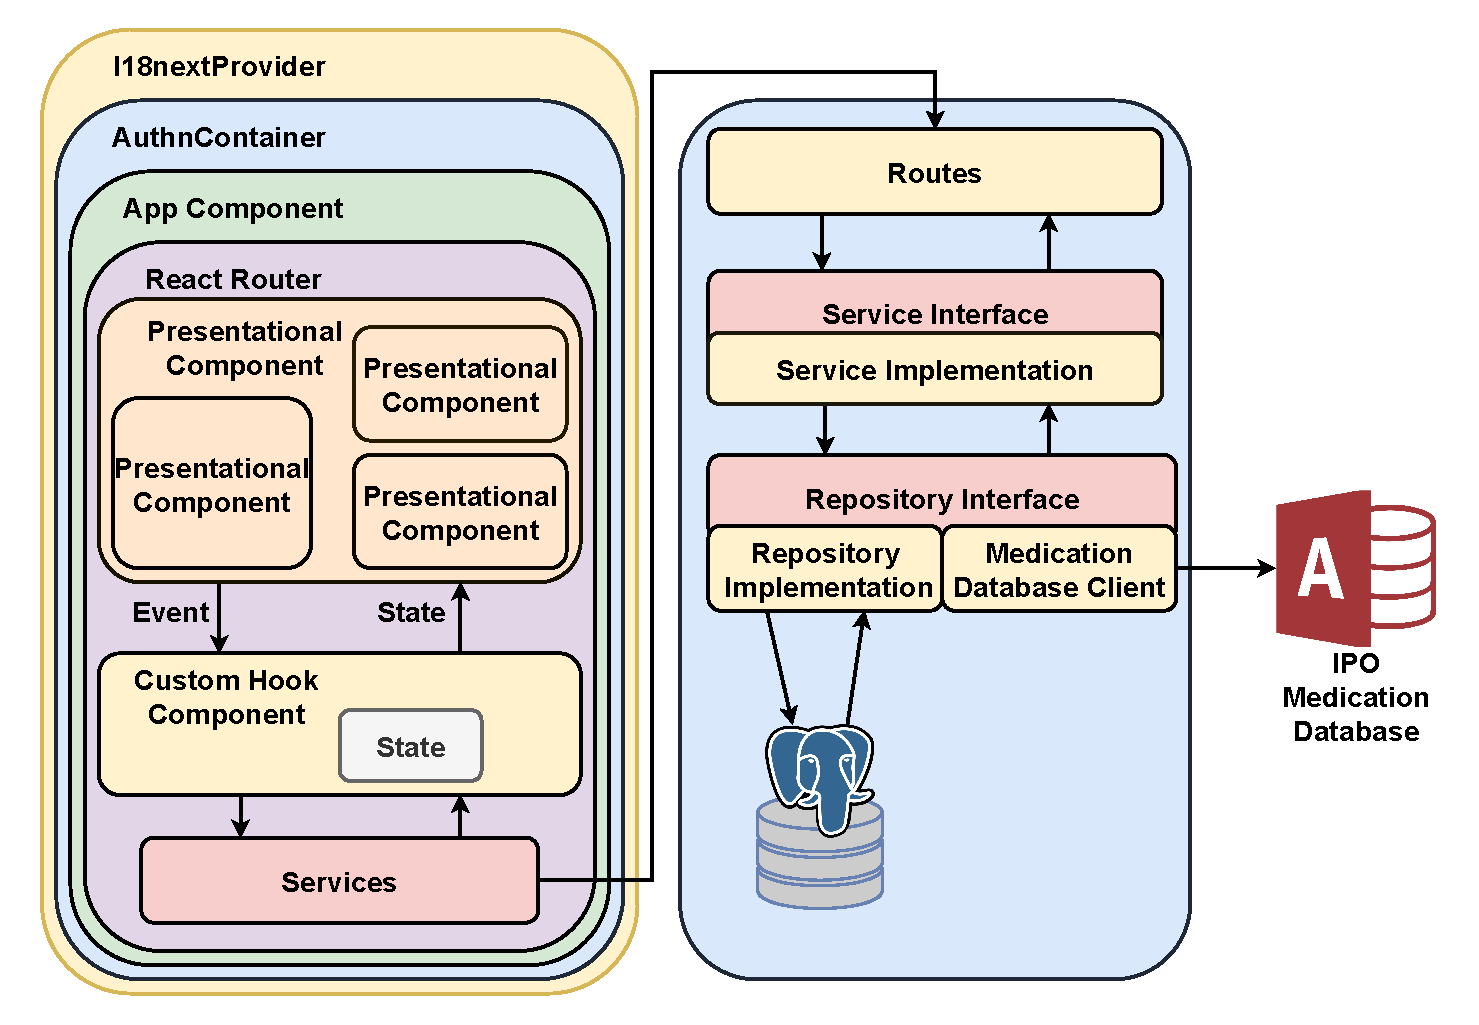
\includegraphics{./figures/Block_Diagram.pdf}}
	\end{center}
	\caption{Block Diagram of our solution.}\label{fig:Block_Diagram}
\end{figure}

\section{Backend} \label{backend}
In this section we will describe the backend.

\subsection{Structure}

The structure for the backend application is as follows:

\begin{itemize}
 \item Program.cs: the entry point of the application;
 \item domain: contains all the domain classes;
 \item repositories: contains the backend repositories that communicate with the ElasticSearch database;
 \item services: contains all the services that, validate and manipulate data, that is received or sent to the routes and repository layer;
 \item routes: contains all the routes of the API which call the adequate service.
 \item utils: contains auxiliary classes and methods.
\end{itemize}

\subsection{Program.cs}

As mentioned before since we're creating a Minimal API, similar to Express.JS, and, as such, server creation is streamlined and the application's functionality is based on middlewares and routing.

The .NET framework makes use of a dependency injection container, aka the service container. As with the Spring Framework, dependencies can have various lifetimes, which in the .NET framework are as follows:
\begin{itemize}
	\item Transient: the dependency is created when needed and disposed thereafter;
	\item Scoped: the dependency is created and maintained in a per request basis;
	\item Singleton: once the dependency is created it's maintained throughout the application's lifetime. 
\end{itemize}

The aforementioned middlewares, which refer to the services and repositories, are registered as services in the container. In our application these services were registered with the Singleton scope, as follows:

\begin{lstlisting}[style=sharpc]
	builder.Services.AddSingleton<IUsersService, UsersService>();
	builder.Services.AddSingleton<IFormService, FormService>();
	builder.Services.AddSingleton<ISearchService, SearchService>();
	
	builder.Services.AddSingleton<IUsersRepository, UsersRepositoryES>();
	builder.Services.AddSingleton<IFormRepository, FormRepositoryES>();
	builder.Services.AddSingleton<ISearchRepository, SearchRepositoryMemory>();
\end{lstlisting}

Using this registration method, for example, when a dependency of type IUsersService is needed, the service container creates a UsersService object to fufill that dependency, hence the inversion of control.

Beyond these, we also used an ElasticClient, however in this service registration, we use a different pattern, instead of using a type and implementation, only the latter was used, this method doesn't allow for multiple implementation, but since there was no need to mock the elastic search database, this feature wasn't needed.

\begin{lstlisting}[style=sharpc]
var nodePool = new SingleNodePool(new Uri("http://localhost:9200"));
var settings = new ElasticsearchClientSettings(
 nodePool,
 sourceSerializer: (_, settings) =>
  {
    return new DefaultSourceSerializer(settings, options =>
      {
        options.Converters.Add(new AnswerConverter());
        options.Converters.Add(new ConditionConverter());
      });
  });
builder.Services.AddSingleton(new ElasticsearchClient(settings));
\end{lstlisting}

According to the Elastic Search documentation, as long as the client instance is a singleton, our application database is thread safe.
\pagebreak

\subsection{Repositories}

The main idea in the repositories is to allow for CRUD operations, ie create users/forms, read users/forms, update users/forms and delete users/forms, on data that is or will be stored in an Elastic Search database. As such the repositories have a dependency on the ElasticsearchClient mentioned before, and they'll use the same client but target different indexes.

\subsubsection{Form Repository}

In the case of the form repository the target indexes will be:

\begin{enumerate}
	\item form : when performing an operation for the form structure, ie the questions and rules;
	\item submissions: when performing an operation for the form's answers;
	\item inconsistencies: when performing an operation for the form's logical fallacies, described in the form of rules;
\end{enumerate}

And this repository will have the following methods:

\begin{lstlisting}[style=sharpc]
public interface IFormRepository
{
	public Task<Form?> GetForm();
		
	public Task<Form> EditForm(Form form);
		
	public Task<bool> SubmitForm(Submission submission, int nic);
		
	public Task<Dictionary<int, Submission>> GetSubmissions();
		
	public Task<Inconsistencies> GetInconsistencies();
		
	public Task<bool> EditInconsistencies(Inconsistencies inconsistencies);
}
\end{lstlisting}

\subsubsection{User Repository}

In the case of the user repository the only target index will be users.

And this repository will have the following methods:
\begin{lstlisting}[style=sharpc]
public interface IUsersRepository
{
	public Task<bool> CheckUserByNicAndPassword(int nic, string hashedPassword);
	
	public Task<bool> AddUser(User user);
	
	public Task<List<User>?> GetUsers();
	
	public Task<User?> GetUserByNic(int nic);
	
	public Task<Boolean> DeleteUser(int nic);
}
\end{lstlisting}

\subsection{Services}
Each service is responsible for managing a certain group of requests, ie the logic to fulfill a request to the /users endpoint will be in the user services. Each service as a dependency on their corresponding repository, which is handled by the service container.

The methods within each service will reflect the possible actions outlined in Chapter ~\ref{cap:problem_description}'s section on uses cases.

\subsubsection{Form Service}

\begin{lstlisting}[style=sharpc]
public interface IFormService
{
	public Task<Result<GetFormOutputModel, Problem>> GetForm();
	
	public Task<Result<Form, Problem>> EditForm(List<QuestionGroupModel> groups, List<RuleModel> rules)
	
	public Task<Result<bool, Problem>> SubmitForm(Dictionary<string,IAnswer> answers, int nic);
	
	public Task<Result<Dictionary<int, Submission>, Problem>> GetSubmissions();
	
	public Task<Result<Inconsistencies, Problem>> GetInconsistencies();
	
	public Task<Result<bool, Problem>> EditInconsistencies(Inconsistencies inconsistencies);
}
\end{lstlisting}
 
 
\subsubsection{User Service}
 
\begin{lstlisting}[style=sharpc]
public interface IUsersService
{
	public Task<Result<Token, Problem>> CreateToken(int nic, string password);
	
	public Task<Result<UserExternalInfo, Problem>> CreateUser(int nic, string password);
	
	public Task<Result<List<UserExternalInfo>, Problem>> GetUsers(string token);
	
	public Task<Result<Boolean, Problem>> DeleteUser(int nic);
}
\end{lstlisting}
\pagebreak

\subsection{Routes}
\subsubsection{Form Routes}
The available endpoints, HTTP method and corresponding operation for all the form routes are available in Table ~\ref{tab:form_endpoints}. 
	
\begin{table}[h!]
	\begin{center}
		\begin{tabular}{l|c|r} 
			\textbf{Endpoint} & \textbf{HTTP Method} & \textbf{Description}\\
			\hline
			/form/structure & GET & Retrieve the last form structure\\
			\hline
			/form/structure & PUT & Updates the form structure\\
			\hline
			/form/submissions & GET & Retrieve all the form answers\\
			\hline
			/form/submissions & POST & Submit form answers\\
			\hline
			/form/inconsistencies & GET & Retrieve the last form's inconsistencies \\
			\hline
			/form/inconsistencies & PUT & Updates the form's inconsistencies\\
			\hline
		\end{tabular}
		\caption{API endpoints related to the form}\label{tab:form_endpoints}
	\end{center}
\end{table}

\subsubsection{User Routes}
The available endpoints, HTTP method and corresponding operation for all the user routes are available in Table ~\ref{tab:user_endpoints}. 

\begin{table}[h!]
	\begin{center}
		\begin{tabular}{l|c|r} 
			\textbf{Endpoint} & \textbf{HTTP Method} & \textbf{Description}\\
			\hline
			/users & POST & Creates a new user\\
			\hline
			/users & GET & Retrieves all the users\\
			\hline
			/users/login & POST & Creates a new access token\\
			\hline
			/users/{nic} & DELETE & Deletes the user with the specified nic\\
			\hline
		\end{tabular}
		\caption{API endpoints related to the user}\label{tab:user_endpoints}
	\end{center}
\end{table}

These routes are then added to the application as follows:

\begin{lstlisting}[style=sharpc]
var group = app.MapGroup("/api");

group.AddUsersRoutes();
group.AddFormRoutes();
\end{lstlisting}

Meaning that the added routes extend the /api endpoint.
\pagebreak

\section{Frontend} \label{frontend}

The frontend application is tasked with data visualization and user interaction. The objective is for the application to provide an intuitive interface for the various users to be able to fulfill the set use cases outlined in section ~\ref{sec:use_cases}.

The frontend is implemented in Typescript and React, and makes use of JSON-Rules-Engine to enforce the form's rules, for further information about these technologies refer to ~\ref{sec:frontend_tech}.

\subsection{Structure}

The frontend structure is as follows:

\begin{itemize}
	\item src: contains the source code of the application;
	\item public: contains the static files of the application;
	\item package.json:  package.json;
	\item tsconfig.json: contains the TypeScript configuration;
	\item routes: contains all the routes of the API which call the adequate service.
	\item webpack.config.js:  contains the Webpack configuration.
\end{itemize}

The src folder is then subdivided into multiple folders/files, each being responsible for a different functionality of the application:

\begin{itemize}
	\item components: contains the components of the pages;
	\item domain: contains the domain objects;
	\item pages:  contains the application's pages, each containing various components;
	\item services: contains the services that communicate with the backend application;
	\item session: contains the code needed to maintain a user session.
	\item utils:  contains general utility functions.
\end{itemize}

It should be noted that, folders within the components folder may contain further utils, containing utility functions that are specially pertinent for that component and shouldn't necessarily be in the general utils. 

Furthermore, besides the aforementioned folders, the src folder also contains an index.tsx and App.tsx files. The index.tsx file is the entry point for the application meanwhile the App.tsx is the main component of the React application.
\pagebreak

\section{Services}

The frontend services are responsible for communicating with the backend application and, as such, each frontend service as a backend counterpart.

To facilitate this communication we used the Fetch API \cite{Fetch_API}, which enables asynchronous resource requests by returning a promise that resolves to a response for that request.

To expedite, and reduce the code for, the api resource requests we created a fetchAPI function that accepts the request parameters and return a promise that will resolve to the requests response, this function can also handle errors if the response's status code isn't in the 200 family.

To further abstract the api calls,  the fetchAPI function was encapsulated within functions that represent specific HTTP methods, such as GET, POST, PUT and DELETE.

\section{Components}

A simplified view of the component tree is presented in Figure ~\ref{fig:reactComponentTree}, in this chapter we'll mainly focus on the AuthnContainer, which manages the session information, the Form, Backoffice and EditFormPage, which are presentational components and the useNewForm and useEditFormPage which are custom hooks.

\begin{figure}[H]
	\begin{center}
		\resizebox{130mm}{!}{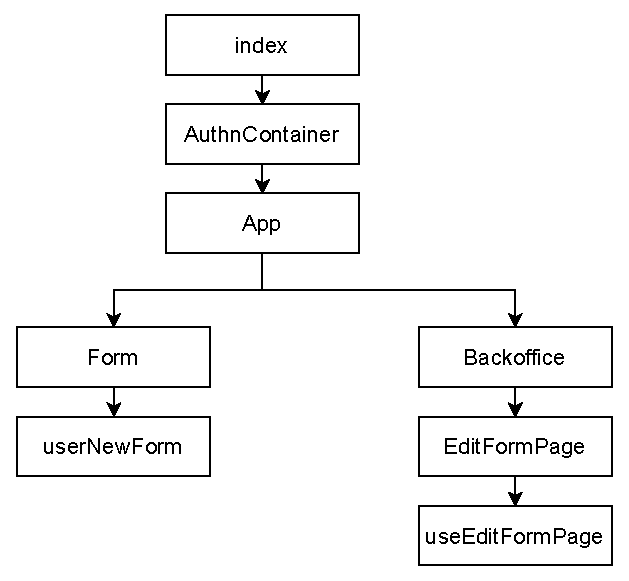
\includegraphics{./figures/reactComponentTree.pdf}}
	\end{center}
	\caption{Simplified React Component Tree.}\label{fig:reactComponentTree}
\end{figure}

\subsection{AuthnContainer}
The AuthnContainer component plays a crucial role in enabling user authentication and consequent storage of the authentication information within the application state.

To do so it uses the React Context API \cite{React_Context_API}, which allows to pass data trough the component tree without having to pass props down manually at every level, thus enabling seamless data sharing between components.

The Session type describe a user's session, ie their name and nic. The SessionManager type acts as a wrapper, containing both the session and the methods to manage it, ie set a session and delete it.

The AuthContainer component wraps it's child components within it's LoggedInContext.Provider, providing the session manager instance and it's methods as the context value, making the authentication information available throughout the component tree.

\subsection{Form}
The Form component is the central component of the application serving as the form page. It leverages the useNewForm hook, which is responsible for retrieving the form structure from the backend and manage it within the application state.

As the user answers the form's the JSON-Rules-Engine is run and, according to the rules in the form, events are triggered, showing or hiding questions, allowing the user to answer the next group of questions or reviewing their answers.

\subsection{EditFormPage}
The EditFormPage component acts a an outlet for the backoffice component page. It leverages the useEditFormPage hook to retrieve the form structure from the backend and manage it's state.

As the user edit's the form's structure the changes are reflected in the hook's state, which is specially difficult given that a question can be a parent, ie it's answer causes another question to appear, and a child, ie it appears as a result of another question's answer.

To solve this issue the hook can reassign questions upon deletion, by finding the group with the parent question and setting the show condition of it's child question as undefined, which means they're automatically shown.


%\newpage
%
%\section{Navigation}
%
%This chapter features a navigation graph, presented in Figure ~\ref{fig:userNavigation}, that describes the UI flow of our platform.
%
%\begin{figure}[H]
%	\begin{center}
%		\resizebox{150mm}{!}{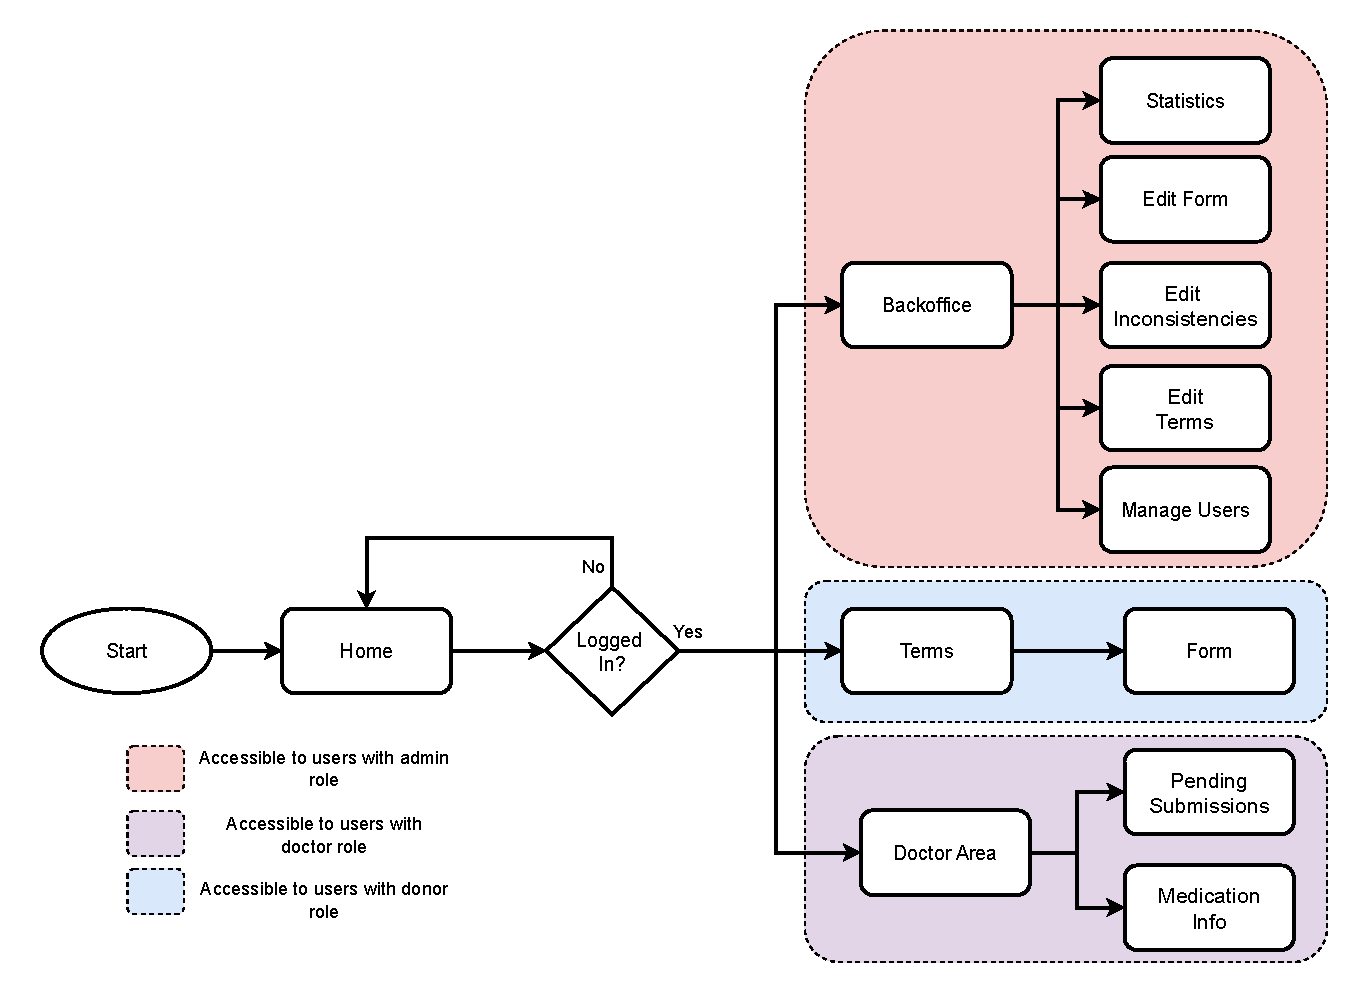
\includegraphics{./figures/userNavigation.pdf}}
%	\end{center}
%	\caption{UI navigation.}\label{fig:userNavigation}
%\end{figure}










